%!TEX TS-program = xelatex
%!TEX encoding = UTF-8 Unicode

% Load Thesis Class
\documentclass{DEIThesis}

\usepackage{pifont}
\usepackage{newunicodechar}
\newunicodechar{✓}{\ding{51}}

\title{Federated Data Analytics for Genomics Data}

\author{Mirco Cazzaro}
\studentId{2076745}

% Advisor
\advisor{Prof. Gianmaria Silvello}

% If you are co-advised
\coadvisor{}
\coadvisorsUniversity{}

\university{University of Padova}
\mastername{Computer Engineering}
\academicYear{2023/2024}

\begin{filecontents*}[overwrite]{\jobname.xmpdata}
    \Title{Federated Data Analytics for Genomics Data}
    \Author{Mirco Cazzaro}
    \Language{en-EN}
    \Keywords{Computer Engineering\sep LaTeX}
\end{filecontents*}

% Document

\begin{document}
    % The front matter (Cover, ToC, Abstract, etc...)
    \frontmatter

    % The main content
    \mainmatter
    
    %!TEX root = ../main.tex

\chapter{Introduction}
\label{chp:intro}

In recent years, the increasing complexity of biomedical data has posed significant challenges to researchers and clinicians. The rapid evolution of data storage systems and the diversity of data models have contributed to these challenges, creating a heterogeneous landscape that is difficult to navigate. This complexity is particularly pronounced in the field of genomics, where the integration and analysis of diverse datasets are crucial for advancing our understanding of genetic diseases and developing personalized medical treatments.
The advent of big data analytics has led to new possibilities for handling large volumes of complex biomedical data. However, the vast diversity of data sources (e.g. relational databases, hierarchical storage systems and graph-based models) necessitates the development of sophisticated data integration frameworks. These frameworks must not only accommodate the different data models but also enable seamless querying and analysis across these models. The need for such frameworks is especially crucial in genomics, where the ability to integrate and analyze data from multiple sources can significantly accelerate research and improve clinical outcomes.
The focus of this thesis is on the design and implementation of a federated data analytics system specifically tailored for the integration of clinical and genomics data. This system is designed to address the challenges associated with integrating heterogeneous data sources, enabling researchers to perform complex queries across multiple datasets without the need for extensive data preprocessing or manual data integration. By leveraging the principles of \ac{OBDA}, the proposed system eases semantic querying capabilities, allowing users to extract meaningful insights from the data more efficiently.
\ac{OBDA} is a powerful paradigm for data integration, particularly in environments characterized by data heterogeneity. Although research activities on \ac{OBDA} started more than 20 years ago, it is still nowadays a subject of discussion in the academic field as well as in the industry, having periodically novel papers discussing both new frameworks or their improvements and their employment in industrial scenarios. \ac{OBDA} allows for the seamless integration of relational databases into an ontology framework, enabling users to perform semantic queries that transcend the limitations of traditional data retrieval methods. The use of ontologies in \ac{OBDA} provides a shared vocabulary and a formalized structure for representing knowledge within a specific domain, which is particularly beneficial in the field of genomics where data is often complex and highly interconnected.
The system developed in this thesis builds upon the \ac{OBDA} paradigm by integrating it into a federated data architecture. This architecture is designed to support the integration of multiple heterogeneous data sources, including relational databases, NoSQL systems, and cloud storage solutions. By creating a unified federated system, the architecture allows for real-time data retrieval and integration, eliminating the need for data deduplication and ensuring that researchers have access to the most current data available.
A key component of this system is the use of a specialized ontology that models the intricate relationships between genomic data and clinical information. The ontology serves as the backbone of the system, enabling the semantic integration of data from diverse sources and facilitating complex queries that would be difficult or impossible to perform using traditional data retrieval methods. The ontology's design is informed by the specific requirements of clinical and genomics research, with a focus on ensuring interoperability and scalability as new data sources and data types are introduced.
The federated architecture proposed in this thesis also incorporates advanced data federation techniques, which are essential for managing the diversity of data sources in genomics. Data federation allows for the creation of a virtual data access layer that abstracts the underlying technical details of each data source, enabling researchers to query data using standard languages like \ac{SQL} without needing to know where the data is physically stored or in what format. This approach not only simplifies the data retrieval process but also minimizes the risks associated with data movement and duplication.
Furthermore, the system is designed with scalability in mind, allowing it to accommodate new data sources as they become available. The system's architecture is flexible enough to integrate these new data sources seamlessly, ensuring that researchers can always work with the most comprehensive dataset possible.
Another critical aspect of the system is its focus on privacy and data security. Given the sensitive nature of clinical and genomic data, especially when data is strictly related to patients' personal information, the system aims to adhere to modern data protection regulations. This is to ensure that while data is integrated and analyzed, it remains protected and secure, ensuring patient privacy and maintaining the trust of the institutions and individuals who provide the data.
The thesis also explores the practical application of the proposed system within the context of the \ac{HEREDITARY} project, a European Union funded initiative focused on integrating multimodal data to advance the understanding of brain diseases. The \ac{HEREDITARY} project represents a real-world application of the federated data analytics system, demonstrating its potential to facilitate complex analyses and drive new insights in biomedical research.
Finally, an extensive benchmarking phase will evaluate the performances of the proposed architecture considering both its strengths as a \ac{DBMS}, analyzing aspects as average execution time and throughput, and the resource consumption of the system, in order to figure out whether such an application adoption may be feasible across diverse hardware environments.
In summary, this thesis presents a comprehensive approach to addressing the challenges of integrating and analyzing heterogeneous clinical and genomics data. Posing its foundations on the \ac{OBDA} paradigm and advanced data federation techniques, the proposed system offers a robust and scalable solution for managing the complexities of biomedical data.

    %!TEX root = ../main.tex

\chapter{Background}
\label{chp:background}

\section{Methodological Background}
\subsection{Resource Description Framework}
The \ac{RDF} is a standard\footnote{https://www.w3.org/RDF/} by the \ac{W3C} designed for data interchange on the web. Its definitive syntax was lastly defined on 2003 \cite{beckett2004rdf}.

\ac{RDF} is based on the idea of making statements about resources, expressed as triples: for example, a triple might consist of "Gene123" (subject) "hasFunction" (predicate) "DNA Repair" (object). These triples are stored in a graph, making \ac{RDF} uniquely suited for modern data analytics where relationships and linkages are crucial: this structure is by design flexible, and it is used to represent information in a way that makes it easier to aggregate, integrate, and manage diverse data from various sources.

The standard utilizes \ac{URI} to ensure that each element in the triple is uniquely identifiable, allowing to link data across different datasets seamlessly. \ac{RDF} also supports literal values and data types, enabling detailed descriptions of properties and values.

In summary, \ac{RDF} provides a robust and flexible framework for describing and interlinking data on the web, which is crucial for any federated data system that aims to integrate diverse data sources effectively.

\subsection{Knowledge Graphs}
Knowledge Graphs represent an innovative way of structuring and querying interconnected data. A \ac{KG} organizes data in a graph format, where entities (nodes) and their interrelations (edges) are defined according to a schema that encapsulates both the entities and the possible links between them. This structure allows not only to better visualize data, but is also very well suited for data exploration and analysis.

Central to the concept of \ac{KG} is the idea of enhancing search and data discovery capabilities beyond simple data retrieval. By semantically linking data entities, \ac{KG} allow for more intuitive and sophisticated queries that are closer to natural language questions. This capability makes them useful in complex domains like biomedical research, where users may need to uncover hidden relationships and patterns among vast datasets.

Furthermore, \ac{KG} well suits in scenarios requiring data integration from disparate sources. They support the combination of structured and unstructured data and they can scale well as new data need to be integrated. This flexibility is crucial in fields such as genomics, where new data attributes and relationships are continuously being discovered and need to be rapidly integrated into existing datasets.

In practice, \ac{KG} are usually powered by technologies such as \ac{RDF} and other standards discussed earlier, leveraging the strengths of these frameworks to ensure robust data handling and scalability.

\subsection{Ontologies}
Ontologies are a shared vocabulary for a particular domain. They serve as a crucial tool in structuring data by defining classes where data entities can be categorized. This classification system not only standardizes data representation but also simplifies the communication between different systems and users by providing a common understanding of the domain.

Ontologies involve the use of first-order logic to define rules about the relationships between different classes. These rules allow for the logical inference of new information from the data that is already known, which can significantly deepen data analysis and querying capabilities. This set of first-order logic rules used to model ontologies composes the \ac{OWL} \cite{mcguinness2004owl}.

With ontologies integrated within a \ac{KG}, it is possible to employ inferential algorithms either at query time or at preprocessing time. This capability enables the derivation of new knowledge that isn't explicitly stated in the data but can be inferred based on the ontological representations.

The use of ontologies in a \ac{KG} is crucial in complex domains like genomics. Here, the ability to infer new relationships and properties can lead to understanding intricate biological connections and processes.

In summary, ontologies provide the foundational structure for managing complex information systems. They not only facilitate a standardized approach to data handling and integration but also enhance the capability of systems to derive and utilize new knowledge effectively.

\subsection{Data Federation} \label{DF}
Data Federation is a technology that organizes data from multiple different and autonomous data sources and makes it accessible under a uniform data model, allowing for real-time data retrieval from various sources without requiring data deduplication. This approach creates a unified data access layer that abstracts the underlying technical details of each \ac{DBMS}. Users can query this virtual layer using standard data querying languages, like \ac{SQL}, without needing to know where the data is physically stored or in what format.

A key strength of Data Federation lies in its capacity to harmonize heterogeneous data sources, ranging from traditional relational databases to modern big data solutions and cloud services. This integration is seamless and dynamic, scaling well as soon as new sources come in, without requiring significant reconfiguration. Such agility is crucial in fields like genomics, where data formats and sources evolve rapidly alongside scientific advancements. Moreover, it minimizes the risks associated with data duplication and movement, such as data loss or corruption. It also ensures that data remains current, reflecting real-time changes without delay. This is particularly valuable for decision-making processes where up-to-date information is critical.

Different existing Data Federation systems may have different characteristics, and the choice of which system suits better certain requirements may depend on many different factors. A recent comparative study on Data Virtualization Systems \cite{DBLP:journals/semweb/GuCLMXXC24} highlights and evaluates diverse features of many systems coming both from the academia as well as enterprise solutions, such as supported query languages, supported data sources, data security, exposed interfaces and software support.

\subsection{Semantic Data Integration}
Semantic Data Integration is an approach that aims to integrate data from a single relational source to an ontology that models a specific domain. This integration is achieved by defining mappings that establish semantic relationships among data entities.

The core idea behind semantic data integration involves establishing a global schema, represented by the ontology, which acts as a blueprint for how data from various sources is viewed and accessed. This ontology defines not just the entities and their attributes but also the relationships and constraints between these entities. The mapping between the ontology (global schema) and the relational data source is critical as it dictates how data is interpreted in a meaningful way.

The concept of Data Integration, firstly introduced without a semantic focus \cite{DBLP:conf/pods/Lenzerini02}, has evolved with research advancements in this field. These advancements have led to the development of tools and mapping languages specifically designed for semantic data integration, laying the groundwork for a paradigm known as \ac{OBDA} \cite{DBLP:conf/ijcai/XiaoCKLPRZ18}.

The \ac{OBDA} framework, that has been precisely formalized \cite{DBLP:conf/aiia/BotoevaCCCX18}, is composed of a chain of procedures that can be summarized as follows:
\begin{enumerate}
    \item input query ${q(\vec{x})}$ is rewritten \cite{DBLP:conf/otm/MakrisGBC10} into ${q'}$ over the virtual ABox ${A'}$ (i.e. the first-order logic specification of the ontology);
    \item the rewritten query ${q'}$ is unfolded using the \textit{mappings} into an \ac{SQL} query ${q^*}$;
    \item the optimized \ac{SQL} query ${q^*}$ is evaluated over the data instance ${D}$ (e.g. a relational \ac{DBMS}).
\end{enumerate}

Figure \ref{fig:OBDAframew} outlines the aforementioned algorithm within a flowchart.

\begin{figure}[ht]
    \centering
    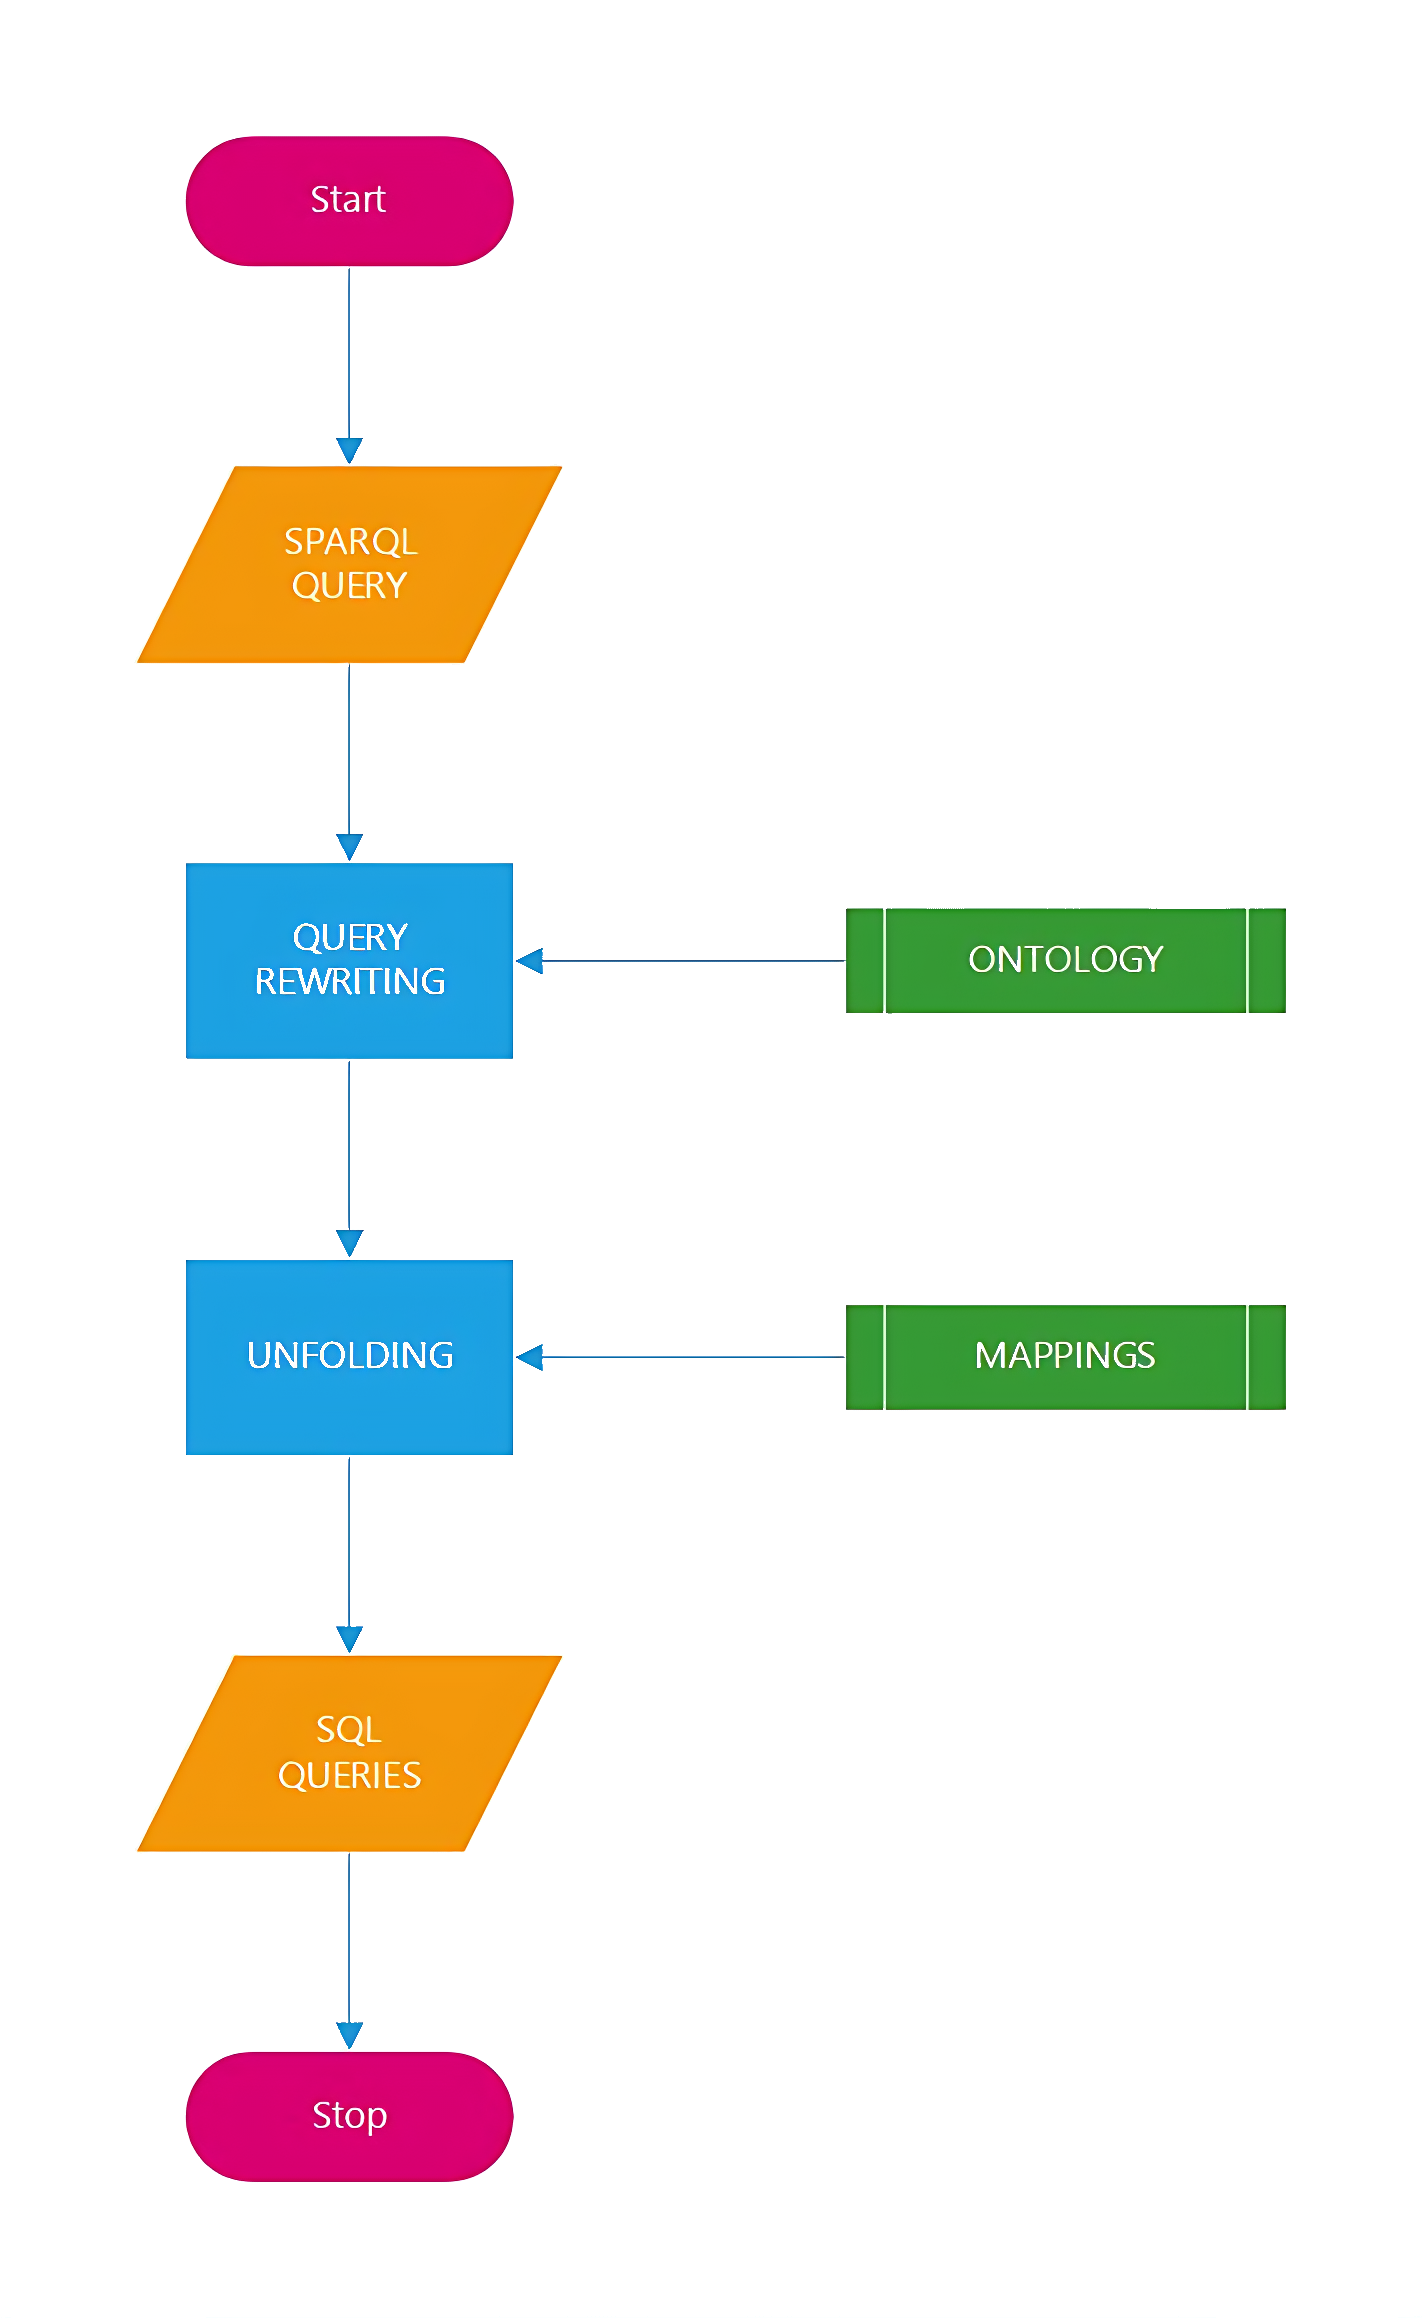
\includegraphics[width=8cm]{res/obda_framework.png}
    \caption{The \ac{OBDA} framework}
    \label{fig:OBDAframew}
\end{figure}


\section{Technical Background}
\subsection{SPARQL Query Language}
\ac{SPARQL}, developed by the \ac{W3C}, is the definitive standard for querying and managing data stored in \ac{RDF} format. 

As a key technology in semantic web applications, \ac{SPARQL} enables sophisticated querying of \ac{KG}, offering a query syntax that often resembles natural language. This user-friendly syntax facilitates intuitive data exploration and manipulation, differently from traditional relational databases that require joining tables to establish relationships.

For instance, as shown in Code \ref{lst:sparql-query}, if a researcher wishes to find all genetic markers associated with a particular trait, a \ac{SPARQL} query might directly reflect the question, “Which patients are associated with genetic markers X?” This parallels natural language questioning closely, making \ac{SPARQL} particularly suited for domains where complex relationships must be understood and explored, such as genomics and biomedical research.

\begin{lstlisting}[language=SPARQL, caption={Example of a \ac{SPARQL} query for genetic markers data.}, label={lst:sparql-query}]
    PREFIX bto: <https://w3id.org/brainteaser/ontology/schema/>
    PREFIX BTO_resource: <https://w3id.org/brainteaser/ontology/resource/>
    
    SELECT ?patient ?FUS ?FUS_mutation
    WHERE { 
       ?p a bto:Patient;
        bto:enrolledIn ?ctp.
        
        ?ctp bto:inClinicalTrial BTO_resource:BrainteaserALSTurin.
        
        OPTIONAL{
            ?p bto:tested ?FUStest.
          ?FUStest bto:hasMutation ?FUS;
                     bto:onGene NCIT:C91852.
            OPTIONAL{
                ?FUStest bto:mutationType ?FUS_mutation.
            }
        }
         
        BIND(SUBSTR((STR(?p)), 48) AS ?patient)
    }
\end{lstlisting}


\subsection{Data Federation Systems}
As discussed in section \hyperref[DF]{2.1.4}, Data Federation Systems are sophisticated software and thus evaluable under many aspects. In this background analysis we will focus on four main aspects, considering their importance as the Data Federation System will be part of a broader framework. In particular, by the aforementioned comparison, we will present three most prominent systems considering:
\begin{itemize}
    \item software support \& documentation;
    \item scalability;
    \item logging capabilities;
    \item performances.
\end{itemize}

These features are also briefly summarized in Tab. \ref{tab:comparison}.

\subsubsection{Denodo}
Denodo\footnote{https://denodo.com/en} is an enterprise virtualization platform that serves as a data federation system, integrating data from diverse sources to provide a unified view without requiring physical data deduplication. It allows for real-time access to structured and unstructured data from various sources including relational, column and No-SQL databases, web \ac{API}, and flat files.

Denodo provides robust security features, including hashing, encrypting functions and user privileges, ensuring that sensitive data is protected according to compliance standards.

Moreover, it utilizes advanced query optimization techniques, such as caching and query rewriting, to enhance performance. These optimizations ensure efficient data retrieval, reducing latency and improving the overall speed of data access across the federated sources.

Although it is highly scalable, capable of accommodating new data sources, and it is provided also with a custom source wrapper template for unsupported data sources, being it an enterprise solution allows for maximum five connections, unless a premium plan is signed.

\subsubsection{Teiid}
Teiid\footnote{https://teiid.io/} is an open-source Java component developed by Red Hat\footnote{https://www.redhat.com/} that provides integrated access to multiple data sources through a single uniform \ac{API}. Rather than a \ac{DBMS}, Teiid is more a query engine for integrating data from multiple sources, accessible both through \ac{API} and \ac{JDBC}/\ac{ODBC} interfaces.

It comes in different shapes: there are Teiid implementations as an Eclipse plugin as well as deployable packages on web containers such as Wildfly and OpenShift.

One of the main issues with Teiid is poor documentation when it is not deployed alongside enterprise solutions (like OpenShift). Moreover, no major releases have been published since four years, and many open issues on the official GitHub repository\footnote{https://github.com/teiid/teiid} are not being addressed.

\subsubsection{Dremio}
Similarly to Denodo, Dremio\footnote{https://www.dremio.com/} is a virtualization platform that serves as a data federation system. Although it is developed within an enterprise context, the standard version, comprehensive of most of the Dremio features, it is \ac{FOSS} under the Apache 2.0 license, combining typical enterprise software robustness with a strong community active on continuous maintenance.

Even if it is possible to use Dremio as a standalone instance (e.g. on a server), it is by design a distributed system and thus it can run on clusters up to more than 1000 nodes. In case of standalone configurations, in linux server environments it is possible to install it using packet managers, but the easiest way is to use the Docker image it comes with.

Dremio makes use of Apache Arrow to enhance processing speeds and reduce latency. Moreover, it optimizes query performance through its advanced query planner and execution engine, which can push down operations to the data source level, minimizing data movement and speeding up response times.

It provides comprehensive security features that include encryption, access controls, and data masking to ensure privacy. It also maintains detailed logs of all queries, which are crucial for compliance purposes in many fields such as the clinical domain, where patient medical data is managed alongside their personal information.

As in Denodo, but under an open-source perspective, it is possible to build custom connectors for unsupported data sources and Dremio. This is realizable through \ac{ARP} connectors: a public repository\footnote{https://github.com/dremio-hub/dremio-sqllite-connector} provides a Maven template, that is customizable for each data source for which a \ac{JDBC} driver is available.

In conclusion, Dremio offers an open-source virtualization system with the typical robustness of enterprise software; it is highly scalable both in the sense of computation distribution over clusters and in the types of supported sources, and it has a comprehensive logging system that suits well for tracking data flow.

\begin{table}[ht]
    \centering
    \begin{tabular}{| p{0.2\linewidth} | p{0.12\linewidth} | p{0.12\linewidth} | p{0.12\linewidth} | p{0.15\linewidth} | p{0.12\linewidth} |}
    \hline
    \textbf{} & \textbf{Support} & \textbf{Free and Open Source} & \textbf{Well Documented} & \textbf{Scalability} & \textbf{Solid Logging Capabilities}\\ \hline
    \raisebox{-0.3\height}{
\includegraphics[width=0.6cm]{res/denodo.png}} Denodo  & ✓ &  & ✓ & ✓ & ✓ \\ \hline
    \raisebox{-0\height}{
\includegraphics[width=0.6cm]{res/teiid.png}} Teiid   &  & ✓ &  &  &  \\ \hline
    \raisebox{-0.3\height}{
\includegraphics[width=0.6cm]{res/dremio.png}} Dremio  & ✓ & ✓ & ✓ & ✓ & ✓\\ \hline
    \end{tabular}
    \caption{Comparative of Data Federation Systems \label{tab:comparison}}
\end{table}


\subsection{OBDA Systems}
\ac{OBDA}, as shown in Fig. \ref{fig:obda_two}, allows to seamlessly integrate a relational source within an ontology, so to add a semantic layer. Research on this specific topic has been performed not only by the academy, but also from Research \& Development branches of big companies, considering the impact on the industry: a preliminary analysis \cite{DBLP:conf/semweb/KharlamovSOZHLRSW14} by Siemens\footnote{https://www.siemens.com/} that lead subsequently to a custom platform, analyzed existing systems. Table \ref{tab:obda_comparison} summarizes the content of this analysis.

\begin{figure}[ht]
    \centering
    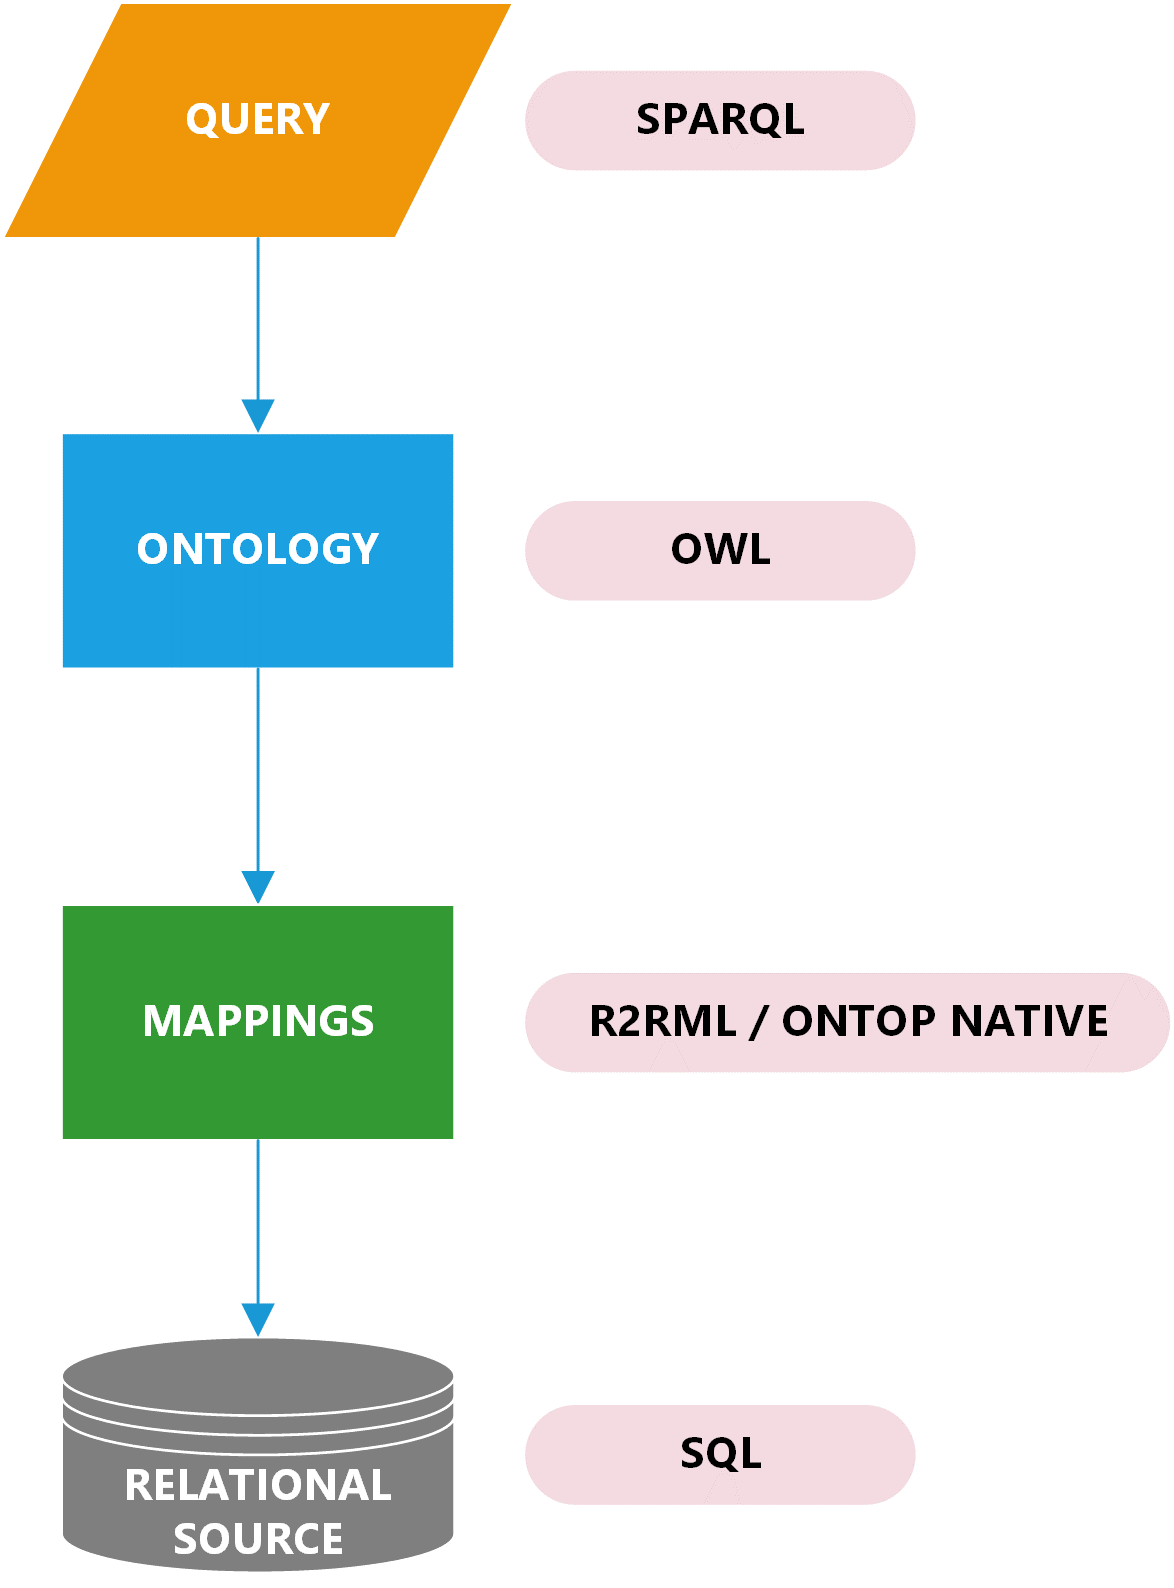
\includegraphics[width=8cm]{res/data_integration.png}
    \caption{The \ac{OBDA} framework}
    \label{fig:obda_two}
\end{figure}


\begin{table}[ht]
    \centering
    \begin{tabular}{| p{0.3\linewidth} | p{0.53\linewidth} |}
    \hline
    \textbf{System} & \textbf{Characteristics} \\ \hline
    Optique (Siemens)  & Supports ontology reasoning; supports both static and streaming relational \ac{DBMS} \\ \hline
    Ontop  & Supports ontology reasoning \\ \hline
    Mastro  & Supports ontology reasoning \\ \hline
    morph-RDB  & Supports ontology reasoning \\ \hline
    D2RQ  & Does not support ontology reasoning \\ \hline
    OntoQF  & Does not support ontology reasoning \\ \hline
    Virtuoso  & Does not support ontology reasoning \\ \hline
    Spyder  & Does not support ontology reasoning \\ \hline
    Ultrawrap  & Does not support ontology reasoning \\ \hline
    \end{tabular}
    \caption{Comparative of \ac{OBDA} Systems \label{tab:obda_comparison}}
\end{table}

Given that ontology reasoning is one of the most important requirements in the \ac{OBDA} approach (without this, using this paradigm would allow just to run queries in \ac{SPARQL} language, without any other real advantage), and considering that the Optique system is an enterprise, on-premise and closed source solution, more in-depth comparisons \cite{DBLP:conf/dlog/NamiciG18} studied Ontop and Mastro. Their comparison can be summarized as follows.

\subsubsection{Mastro}
By our knowledge, Mastro \cite{DBLP:journals/semweb/CalvaneseGLLPRRRS11} was the first \ac{OBDA} tool, developed at La Sapienza University of Rome. It supports a subset of \ac{SPARQL} queries and integrates a custom XML-based mapping syntax.
Mastro's mappings were not initially compliant with R2RML standards, which was a strong limitation in standard \ac{OBDA} environments. The tool used a complex system of view predicate mappings, which may affect its adaptability to standardized environments. Although recent updates have integrated R2RML support, the system's architecture still lacks certain optimizations due to its design constraints. For instance, Mastro cannot perform advanced semantic query optimizations because it does not support detailed data constraints in its mappings. This limitation could lead to less efficient query processing and increased execution times, especially with complex queries involving multiple joins or extensive data operations.
Moreover, Mastro is less efficient handling of datatype operations and IRI constructions within \ac{SQL}, leading to potential slowdowns in query processing.

\subsubsection{Ontop}
Ontop \cite{DBLP:conf/sebd/CalvaneseCKKKLR15} is an open-source and well maintained \ac{OBDA} framework developed at the Free University of Bolzano. It is compliant with \ac{W3C} standards, including R2RML for ontology mapping, \ac{OWL} for ontology representation, and \ac{SPARQL} for querying. Ontop is designed for high-performance query answering over virtualized \ac{RDF} graphs.
Ontop provides an efficient query answering system that leverages R2RML mappings and supports comprehensive optimizations. The system uses advanced query rewriting techniques, which are highly effective in reducing query complexity and execution time. Ontop's strengths are particularly evident in its handling of complex \ac{SPARQL} queries, where it efficiently translates these into \ac{SQL}, utilizing T-mappings and database integrity constraints for optimization.
Regardless of its adherence to standards, Ontop comprises also a custom mapping language (Ontop Native Language).

The comparison between the two systems has been performed in two different scenarios. In general, Mastro shown faster responses in scenarios requiring extensive in terms of timings, while Ontop performs better in scenarios where a considerable number of mappings is involved for unfolding a certain query.
This means that a choice on which system fits better depends on how constraining are timings in the query processing phase and on how many mappings have to be unfolded on average, that strictly depends on the heterogeneity of the underlying relational source.

\subsection{Triple Stores}
Triple stores are database management systems specifically designed to store and retrieve triples through semantic queries. Triple stores typically ingests \ac{RDF} files that contains IRI's in the usual format of subject, predicate, object. These systems are optimized for storing vast amounts of triples and efficiently handling complex queries that involve traversing relationships across a network of data. Triple stores support \ac{SPARQL}, enabling semantic queries that are essential for applications in data integration, knowledge management, and semantic web projects.
Many comparisons, especially in the biomedical field \cite{DBLP:journals/entropy/CanSBU17}, among different triple stores systems analyze their performances under different point of view such as the volume of ingested data, the implementation of an ontology within the \ac{KG}, and the language used to represent it (\ac{RDF}, RDFS, \ac{OWL}, etc.).
For the purposes of this project, where materialized triples are not used, GraphDB has been selected due to its integration with Ontop. This integration allows GraphDB to support virtual graph functionalities, meaning it can perform \ac{SPARQL} queries over non-RDF relational data by translating these queries into \ac{SQL} through Ontop's engine. This scenario eliminates any particular requirements from the triple store system regarding the query processing phase, considering that the task will be accomplished by the underlying \ac{OBDA} system.

\subsubsection{GraphDB}
GraphDB is a robust, enterprise-ready triple store that excels in handling large volumes of data and complex queries. Developed by Ontotext\footnote{https://www.ontotext.com/}, GraphDB is designed to facilitate efficient data integration, knowledge discovery, and semantic analytics. It uses \ac{RDF} for data representation and \ac{SPARQL} for querying, supporting seamless transitions between different data formats and query languages.
GraphDB's integration with Ontop for virtual \ac{RDF} stores and its robust performance metrics make it an ideal choice for projects that require dynamic semantic data integration without the overhead of materialized triples. Its capabilities ensure that it is not only a powerful tool for \ac{RDF} data management but also a flexible solution for broader data integration challenges in semantic environments.
    %!TEX root = ../main.tex

\chapter{Related Works}
\label{chp:related}

Performing federated analytics tasks over genomics data requires a robust architecture composed by different layers: a federation layer that allows for multiple streaming connections with diverse and heterogeneous sources (relational, no-SQL and columnar \ac{DBMS}s); a virtualization layer that exposes "virtual" relational views of non-materialized data; an integration, ontology-based layer, so to add a semantic layer to the virtualized relational views, given the importance of exploring complex relationships among genomics data.

This approach has been formalized under the concept of \ac{OBDF} \cite{DBLP:conf/icde/GuCPLMX24}, and it is represented in Fig. \ref{fig:obdf}. As far as we know, no existing off-the-shelf system implementing this framework has ever been released: who intends to apply this architecture design have to manually install different components choosing among diverse competitors, and combining them together, dealing with possible underlying platform incompatibilities. Moreover, having no off-the-shelf solutions implies no solutions specifically tailored and optimized for dealing with genomics data.

\begin{figure}[ht]
    \centering
    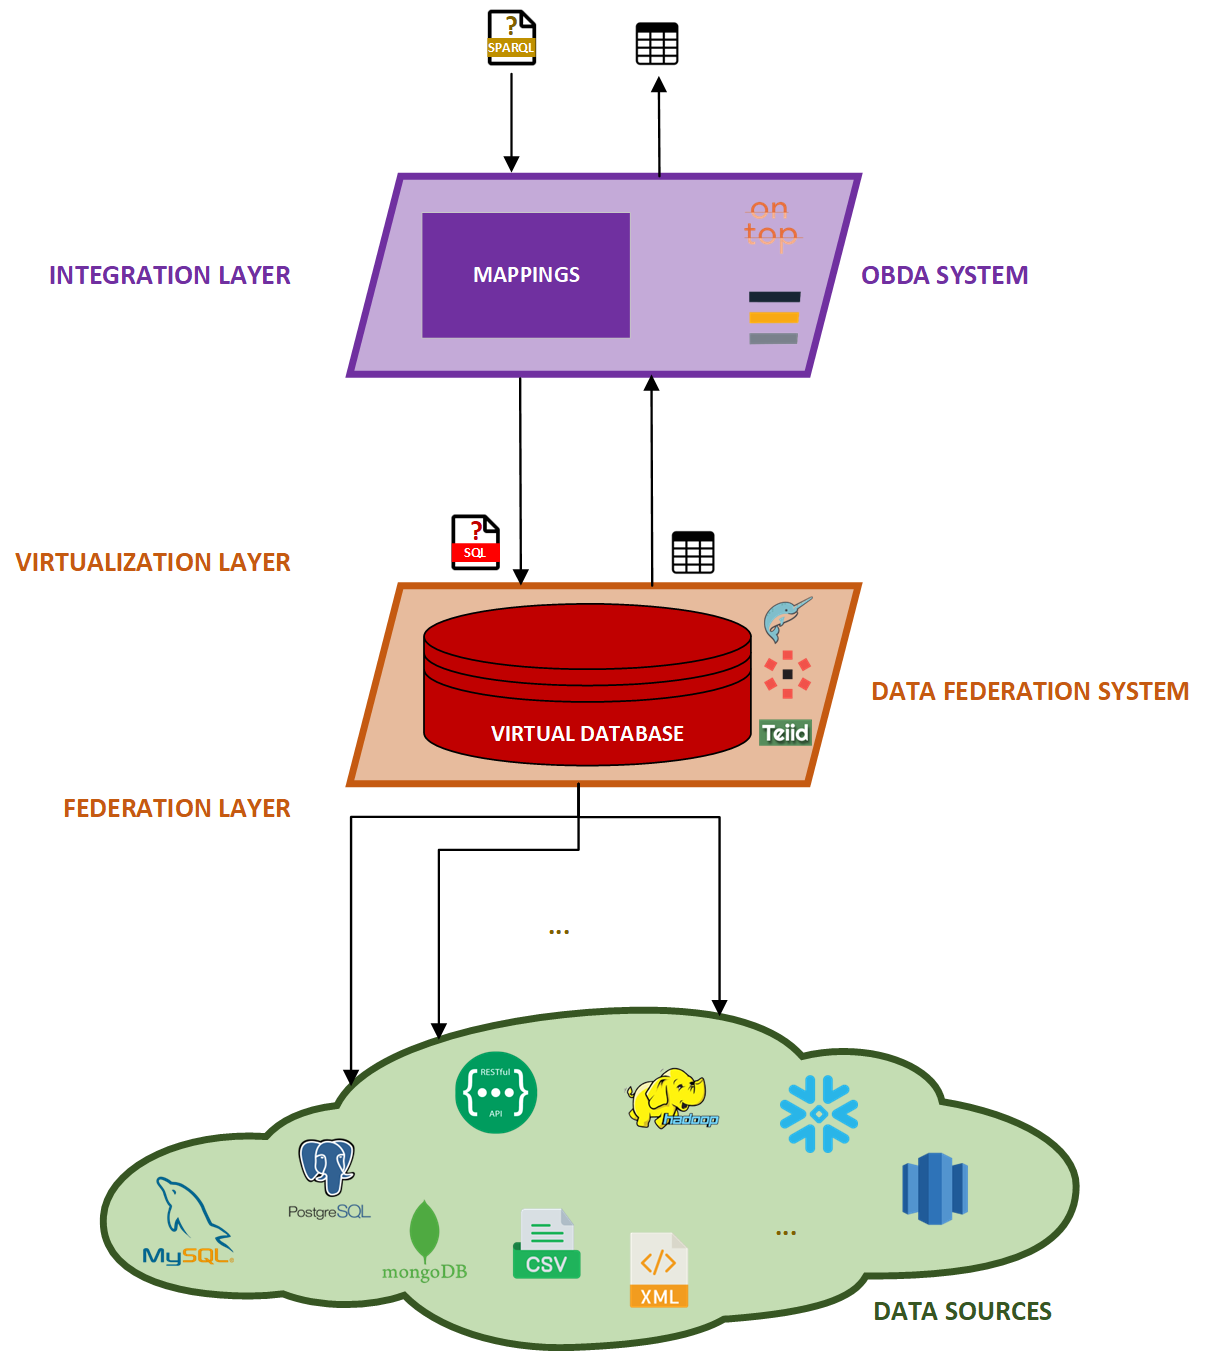
\includegraphics[width=10cm]{res/Drawing4.png}
    \caption{OBDF approach}
    \label{fig:obdf}
\end{figure}

Nonetheless, similar design proposal have been implemented in order to address both research questions as well as enterprise requirements. In this section, we will briefly discuss two solutions, one for each environment, analyzing them in details highlighting strengths and weaknesses.

\section{BigDAWG}
As an example addressing research questions about managing heterogeneous data we have BigDAWG \cite{DBLP:conf/hpec/GadepallyCDEHKM16}, developed under the Intel Science and Technology Center on Big Data. BigDAWG's architecture is composed of four layers: the base layer, the island layer, the main BigDAWG layer, and the application layer. Each layer serves a distinct purpose, from managing diverse physical data stores to facilitating user interaction through applications. This multi-layered approach allows BigDAWG to support various data models and query languages, thus offering a robust solution for cross-database queries and operations.
While traditional systems such as Garlic and IBM DB2 have demonstrated the capability to handle data across different storage systems using a unified interface, BigDAWG distinguishes itself by its comprehensive support for "islands" of different data models. This island approach not only supports operations across various data types but also enhances performance by optimizing queries based on the data model and the underlying database engine. This feature is critical in environments where performance and response times are crucial, such as in medical or real-time analytics applications.
Despite its advanced architecture and capabilities, BigDAWG is not without challenges. It is not available as an off-the-shelf solution; rather, it require certain levels of expertise if someone intends to install it or develop new islands modules. This means that significant effort would be required to adapt it to specific operational needs. Additionally, there is limited literature and empirical studies on its deployment in real-world scenarios, which poses doubts about considering its implementation.
In summary, while BigDAWG represents a significant advancement in the field of database management systems, its practical application is limited by the prototype nature of its current implementation and the lack of extensive real-world testing. Future research could focus on reducing the barrier to its adoption, refining its architecture based on operational feedback, and expanding its use cases across different scenarios to fully realize its potential.

\section{Optique}
Optique \cite{DBLP:journals/ws/KharlamovMSXKR19}, developed by Siemens, exemplifies an implementation of OBDA tailored to the industrial applications. Unlike conventional OBDA systems which typically focus on static data, Optique is designed specifically to handle both streaming and static data. This dual capability is crucial for environments like Siemens, where real-time data from sensors needs to be integrated with historical data for comprehensive analysis and monitoring.
Optique comprises many technologies: \ac{STARQL}, A language that supports complex queries over streaming and static data at the same time; ExaStream, A backend system optimized for low-latency queries on high-velocity streams; OptiqueVQS (Visual Query System), a component that improves usability by enabling users to formulate queries without prior knowledge of query languages.
Although it has advanced capabilities, Optique remains a proprietary system not available for public use, which limits its adoption outside Siemens. This exclusivity may impede broader validation and benchmarking against other OBDA systems in real-world settings.
    %!TEX root = ../main.tex

\chapter{Context of the Work}
\label{chp:context}
    %!TEX root = ../main.tex

\chapter{System Architecture}
\label{chp:architecture}

As discussed in Chapter \ref{chp:related}, there exist no off-the-shelf solution implementing the \ac{OBDF} paradigm. This implies that for the specific task of dealing with clinical and genomics data, it is necessary to design a system architecture, choosing components in such a way that the whole architecture results in being solid, privacy-oriented (with strong logging capabilities), and being capable to manage genomics data.
This chapter will firstly discuss the overall proposed architecture, that retraces the one presented in previous chapters. Subsequently, each layer will be presented in details, outlining how each components have been configured, reporting eventual code snippets. In order to better describe the source heterogeneity of data that may occur in contexts such as clinical and genomics, available relational data have been distributed among different sources.

\section{System Architecture Design}
\begin{figure}[ht]
    \centering
    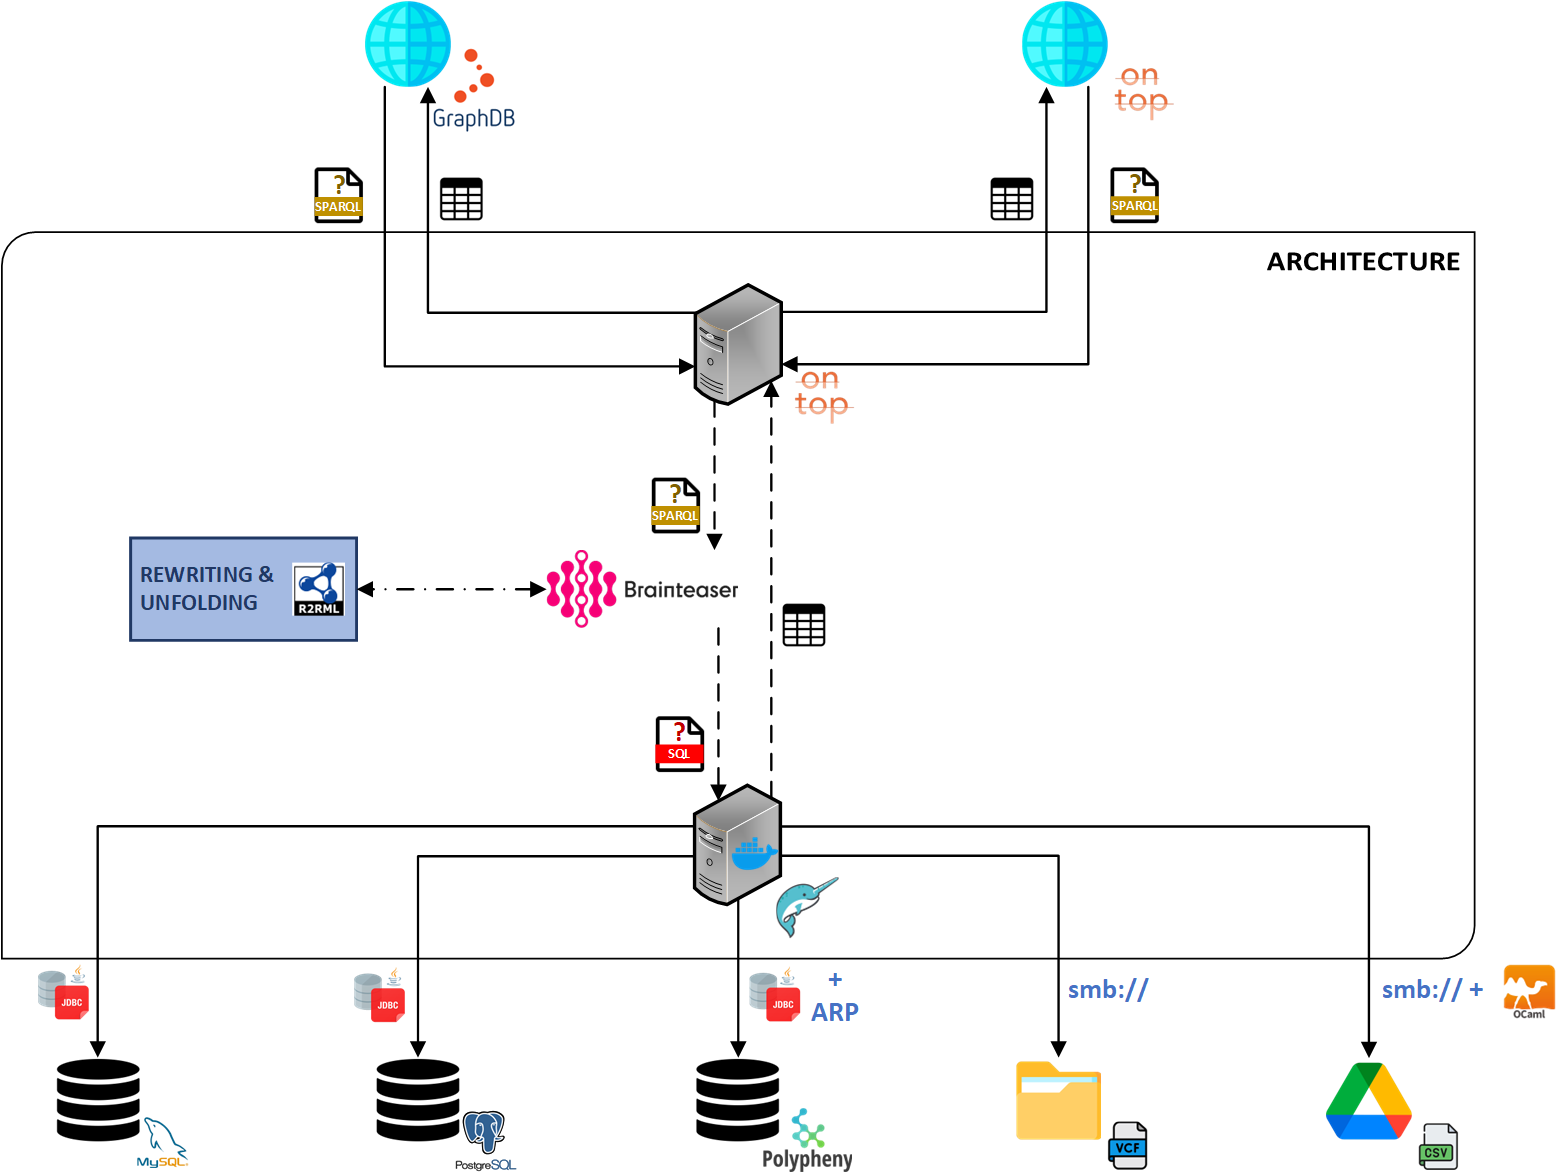
\includegraphics[width=15cm]{res/Drawing1.png}
    \caption{Proposed System Architecture}
    \label{fig:mirco_arch}
\end{figure}
The proposed architecture described in Fig. \ref{fig:mirco_arch} implements the \ac{OBDF} framework. It adopts Ontop as its semantic data integration layer and Dremio as its data federation layer. 

Briefly, Ontop have been chosen because it natively supports two high level mapping languages, that gives more freedom on their optimization, without the need to appeal to low level \ac{DL} languages, it is open-source and well maintained by the Free University of Bolzano data integration team, it comes embedded in GraphDB that offers solid \ac{API}s, and it comes even with an embedded web endpoint.

Dremio have been chosen as the virtualization and federation layer because, as discussed in the Chapter \ref{chp:background}, it is an open-source, robust and scalable software influenced both from its enterprise nature and from a consistent community providing contributions. Moreover, within its installation methods, it is possible to set it up through a Docker image: this may set the basis for the architecture packaging, expanding the image to other software components.

The semantic integration requires an ontology well describing the domain of clinical and genomics data. Considering the reusability principle that stands at the basis of the semantic web, we identified the Brainteaser ontology\footnote{https://brainteaser.dei.unipd.it/ontology/} as suitable for accomplishing this task. 

\section{Data Sources}
Given the relational nature of available data, we distributed it among five different platforms, so to exploit the federation capabilities of the data federation layer. The choice of the sources has been guided also by surveying commonly used ones in the biomedicine field in contexts like research and hospital diagnostic. As we will discuss, they encompasses more structured \ac{DBMS}s as well as simple \ac{CSV} files. We also included a novel \ac{DBMS} system, so to investigate how new, unknown data sources can be federated as soon as they figure out.

\subsection{MySQL}
MySQL\footnote{https://www.mysql.com/it/} is one of the most widely used relational \ac{DBMS} (DBMS) in the world. It is a \ac{FOSS} solution now distributed by Oracle\footnote{https://www.oracle.com/it/}. It is extensively employed across a variety of applications, from small personal projects to critical enterprise environments. In our system architecture, we've chosen MySQL considering its extensive adoption, possibly also in application softwares used in clinics and hospitals to collect patients data. 
In our environment, MySQL's role is to store part of the structured clinical data presented in Chapter \ref{chp:context}. 
The interfacing between MySQL and our data federation layer, Dremio, is performed through MySQL's JDBC connector. This setup allows Dremio to access and query MySQL data seamlessly.
No special modifications or configurations were required to integrate MySQL with Dremio, thanks to Dremio's native support for MySQL. We simply established a new data source within Dremio by specifying the connection parameters.

\subsection{PostgreSQL}
PostgreSQL\footnote{https://www.postgresql.org/} stands out as a widely adopted open-source relational \ac{DBMS}. It is particularly adopted within the research community due to its robustness, advanced features, and strong compliance with SQL standards. Many research institutions and academics prefer PostgreSQL for its extensive capabilities in managing complex data types and its support for sophisticated data manipulation operations. We considered PostgreSQL eligible to be a data source due to its common adoption in research contexts as a data collector.
Again, PostgreSQL's role in our environment is to store another portion of the structured clinical data presented in Chapter \ref{chp:context}.
Just like with MySQL, integrating PostgreSQL with Dremio did not require any specific modifications or additional configurations.

\subsection{Polypheny}
Polypheny \cite{DBLP:conf/bigdataconf/VogtSS18} is an open-source polystore system designed to support diverse data models including relational, document, and graph data. It is engineered to handle mixed workloads and various query languages, making it a versatile platform suitable for dynamic data environments.
In our architecture, we consider Polypheny not just as a standalone polystore but as a potential low-level federator under our main data federation layer managed by Dremio. This perspective is particularly useful because it allows us to leverage Polypheny's ability to handle multiple data models, thus enriching the flexibility and capability of our overall data management system.

\subsubsection{Custom ARP Connector Development}
Unlike the straightforward integrations with MySQL and PostgreSQL, incorporating Polypheny required a more sophisticated approach. We performed this task not only to include Polypheny as one of our data sources but also as a proof of concept about the actual possibility of developing custom ARP connectors.
Dremio's Advanced Relational Pushdown (ARP) framework offers a powerful mechanism to extend Dremio's capability to interact with various data sources by intefacing Dremio's internal query representations into the native query language of the target data source.
For Polypheny, we developed a custom ARP connector to ensure interaction between Dremio and Polypheny. The connector we developed is open-source and available for the community, which can be found at our GitHub repository \footnote{https://github.com/mircocazzaro/dremio-polypheny-arp}.
These connectors rely on the target source having a \ac{JDBC} driver and accepting SQL as a query language, so to have an interface to dialog with.

\subsubsection{Connector implementation Details}
The custom ARP connector was implemented to translate SQL queries from Dremio into the query formats that Polypheny can execute directly.
The ARP plugin template\footnote{https://github.com/dremio-hub/dremio-sqllite-connector} consists of a Java Maven project, that has to be compiled, packed within a \ac{JAR} file and injected, together with the target source \ac{JDBC} driver, into the running Dremio instance.
To customize the template, two files needs to be customize: the storage plugin configuration, which is a Java class \ref{lst:polypheny-arp}, and the plugin ARP file, which is a YAML\footnote{https://yaml.org/} file.
The storage plugin configuration file tells Dremio what the name of the plugin should be, what connection options should be displayed in the source UI, what the name of the ARP file is, which JDBC driver to use and how to make a connection to the JDBC driver.
The ARP YAML file is what is used to modify the SQL queries that are sent to the JDBC driver, allowing you to specify support for different data types and functions, as well as rewrite them if tweaks need to be made for your specific data source. 

\begin{lstlisting}[language=JAVA, caption={The storage plugin configuration file}, label={lst:polypheny-arp}]
/* ... */

@SourceType(value = "POLYPHENY", label = "POLYPHENY")
public class PolyphenyConf extends AbstractArpConf<PolyphenyConf> {
  private static final String ARP_FILENAME = "arp/implementation/polypheny-arp.yaml";
  private static final ArpDialect ARP_DIALECT =
      AbstractArpConf.loadArpFile(ARP_FILENAME, (ArpDialect::new));
  private static final String DRIVER = "org.polypheny.jdbc.Driver";

  @NotBlank
  @Tag(1)
  @DisplayMetadata(label = "Polypheny host <HOST:PORT>")
  public String database;

  /* ... */

  @Tag(2)
  @DisplayMetadata(label = "Record fetch size")
  @NotMetadataImpacting
  public int fetchSize = 200;

  @Tag(6)
  @DisplayMetadata(label = "Polypheny User Name")
  public String username = "pa";

  @Tag(7)
  @DisplayMetadata(label = "Polypheny Password")
  public String password = "";

  @Tag(4)
  @DisplayMetadata(label = "Maximum idle connections")
  @NotMetadataImpacting
  public int maxIdleConns = 8;

  @Tag(5)
  @DisplayMetadata(label = "Connection idle time (s)")
  @NotMetadataImpacting
  public int idleTimeSec = 60;

  @VisibleForTesting
  public String toJdbcConnectionString() {
    final String database = checkNotNull(this.database, "Missing database.");

    return String.format("jdbc:polypheny://%s", database);
  }


  private CloseableDataSource newDataSource() {
    return DataSources.newGenericConnectionPoolDataSource(DRIVER,
      toJdbcConnectionString(), username, password, null, DataSources.CommitMode.DRIVER_SPECIFIED_COMMIT_MODE,
            maxIdleConns, idleTimeSec);
  }
}
\end{lstlisting}

With respect to the storage plugin configuration Java class \ref{lst:polypheny-arp}, being Polypheny still an embryonic project not allowing for user management, but rather having a default user "pa" with empty password, fields are pre-filled with default values. The class specification is then interpreted at run time from Dremio, setting up a form with input fields corresponding to each @DisplayMetadata annotation.
The DRIVER static and immutable variable contains the class path of the Polypheny \ac{JDBC} driver. The newDataSource() method is invoked at form submission, setting up the connection to the Polypheny instance.

\subsection{NAS Folders}
Dremio offers native support for a variety of "relational" file types such as \ac{CSV}, Excel, \ac{JSON}, and \ac{VCF}. These files may be physically moved within the Dremio instance, but losing any streaming capability, or by attaching a \ac{NAS} source to it. In fact, Dremio integrates a connector to local folders, reading supported files within them. The name \ac{NAS} on this typology of data source is ambiguous: the term refers to storage units usually located within the same \ac{LAN} of one or more hosts accessing it, while in Dremio is used to generically refer to a folder to which it can access.
This in practice means Dremio can browse local folders: thus, if NAS shared folders are mounted within the Dremio server through the \ac{SMB} protocol, they can be browsed as well.
In Linux environments where the standalone version of Dremio is used, its daemon must have permission to read these folders; in environments where the Docker image is employed, where a clear separation between the host file system and the Docker context occurs, folders and \ac{NAS} shares must be mapped. This is obtained with Docker Volumes\footnote{ https://docs.docker.com/storage/volumes/}, and in particular the “Host Volume” paradigm.
\begin{lstlisting}[language=bash, caption={Docker command to run a Dremio container with a Host Volume}, label={lst:docker-host-volume}]
$ docker run -v NAS_PATH/folder:/opt/dremio/folder -p 9047:9047 -p 31010:31010 -p 45678:45678 -p 32010:32010 --name hereditary_dremio dremio/dremio-oss
\end{lstlisting}
For the purposes of our project, we have utilized the \ac{NAS} data source to store a portion of our genomics data. Specifically, we have chosen to include data in \ac{VCF} files. \ac{VCF} is a text file format generally used in bioinformatics for storing gene sequence variations.

\subsection{Google Drive}
Google Drive is a widely used cloud storage service offered by Google that allows users to save files and access them from any device connected to the internet. Users can store documents, spreadsheets, and presentations, collaborate with others, and have all their work backed up safely.
We chose to consider Google Drive as a data source for our system architecture primarily because of its widespread use in various contexts, including scenarios where Google Sheets are frequently adopted for data collection and management. Google Sheets, part of the Google Drive suite, is particularly popular in both academic and industrial settings for its ease of use and collaborative features.
The approach to integrating Google Drive is identical to that of the \ac{NAS} system, as long as Google Drive is adapted to a local host folder. This adaptation allows Dremio to interact with Google Drive as if it were interacting with local file systems, thereby simplifying access and manipulation of data stored in Google Drive.
The adaptation of Google Drive to a local system is facilitated by a tool known as google-drive-ocamlfuse\footnote{https://github.com/astrada/google-drive-ocamlfuse}, which provides a FUSE-based file system backed by Google Drive. This tool was built using OCaml, a functional programming language known for its expressiveness, efficiency, and robustness. OCaml is utilized to handle the logical operations and data structure management, ensuring that the application runs efficiently and securely. \ac{FUSE} is a software interface for Unix-like computer operating systems that lets non-privileged users create their own file systems without editing kernel code. This is used in google-drive-ocamlfuse to mount Google Drive as a file system on the user's computer.
\subsubsection{Adaptation of Google Sheets}
With the google-drive-ocamlfuse tool, Google Sheets can be adapted to local Excel files, which are natively supported by Dremio. This adaptation is crucial because it allows Dremio to perform operations on Google Sheets just as it would on local Excel files, enabling seamless data processing and integration without needing to convert or move data physically.
\subsubsection{Configuration and Usage}
Configuring google-drive-ocamlfuse involves setting up Google Drive as a mounted file system. Once mounted, the Google Drive folder behaves like any other directory on the local system.
\begin{lstlisting}[language=bash, caption={google-drive-ocamlfuse Tool installation procedure}, label={lst:ocamlfuse}]
# Installation of google-drive-ocamlfuse
$ sudo add-apt-repository ppa:alessandro-strada/ppa
$ sudo apt-get update
$ sudo apt-get install google-drive-ocamlfuse

# Authentication and mounting
$ google-drive-ocamlfuse
$ mkdir ~/google-drive
$ google-drive-ocamlfuse ~/google-drive
\end{lstlisting}
We used the Google Drive data source to store the remaining part of \ac{VCF} genomics data.


\section{Federation and Virtualization Layer}
At the bottom of our system architecture we do have a software component that encompasses both the federation and virtualization functionalities. In fact, this component not only allows to seamlessly connecting to multiple diverse data sources, but also serves as a virtualizator by creating unmaterialized virtual views of the integrated data. This dual functionality is essential in our scenario for efficiently managing data access and manipulation across the disparate systems involved in our project.
\subsection{Role of Federator}
As a federator, this layer allows for extensive connectivity, facilitating interactions with various types of data sources ranging from traditional relational databases like MySQL and PostgreSQL to modern polystore systems such as Polypheny, and even cloud-based storage solutions like Google Drive. The ability to federate across these diverse sources means that data, regardless of where it is stored or in what format, can be accessed and queried as if it were located within a single, homogeneous database.
\subsection{Role of Virtualizator}
On the virtualization side, the layer enables the creation of virtual views that do not require materialization. These views treats relations exposed from underlying data sources as if they are actual tables within the same database schema: as Fig. \ref{fig:virtual} shows, this implies that these tables can be joined together and thus expose the most meaningful information to the upper architecture layers. Moreover, tables can be joined with pre-defined views, further enhancing the virtualization capabilities. No data is physically stored within this layer, but rather queries coming into this layer are dynamically interpreted and delegated to the source \ac{DBMS}s. This approach ensures that the most current data is always presented to the user or application, without the overhead and delay associated with physical data integration. In the subsequent sections, a diagram will be included to illustrate how these virtual views are structured and managed within our system.
\begin{figure}[ht]
    \centering
    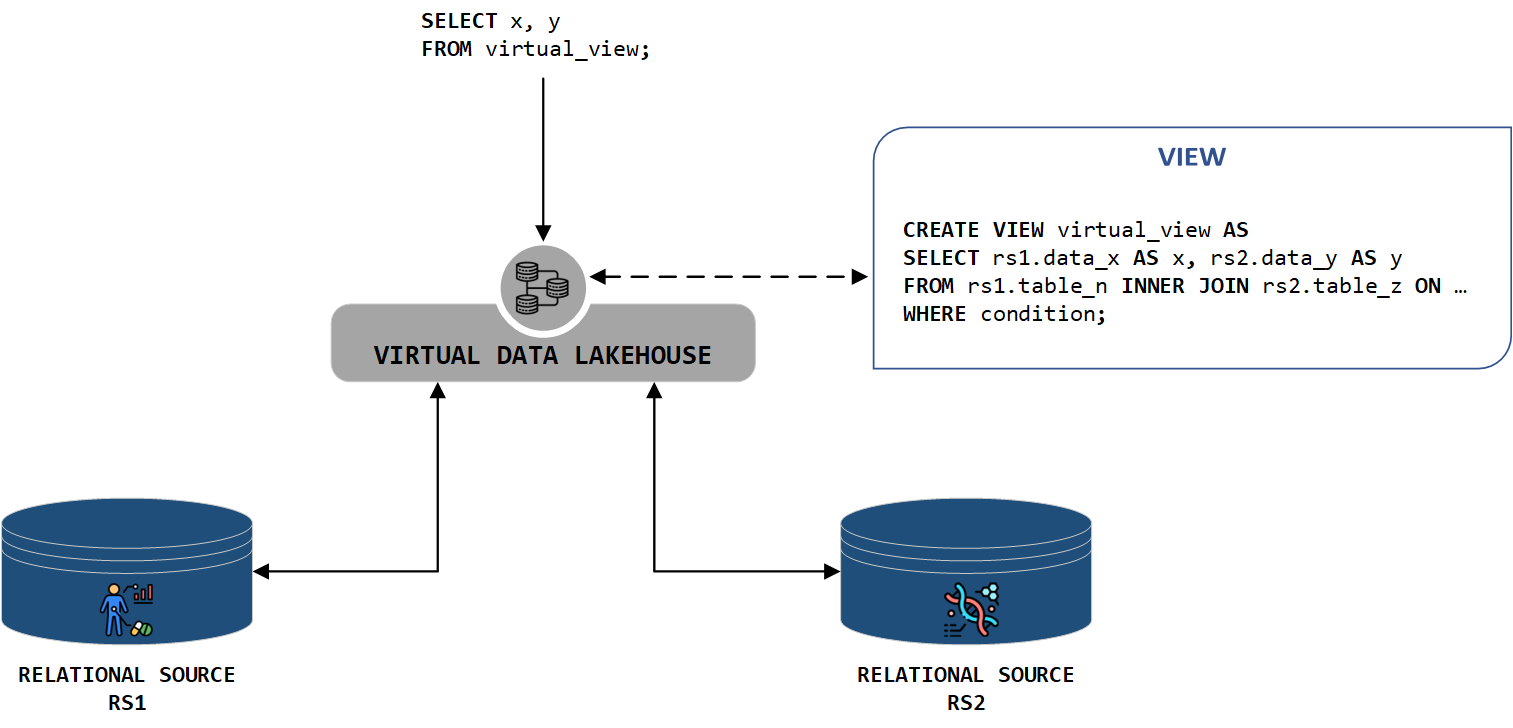
\includegraphics[width=15cm]{res/Drawing2.png}
    \caption{Virtual Views}
    \label{fig:virtual}
\end{figure}
\subsection{Focus on Dremio}
\subsubsection{Web Interface}
One of the main features of Dremio is its user-friendly web interface, which provides a graphical user interface (\ac{GUI}) that simplifies the process of data management. This interface is particularly beneficial for defining and managing virtual views. As shown in Fig. \ref{fig:screenshot} users can interact with the system through the web interface to run queries, visualize query results and configure the system settings.
\subsubsection{Defining Virtual Views}
Within Dremio's web interface, users can create and manage virtual views. These datasets do not store any data themselves but instead provide a virtual schema on top of physical data stored across different sources. Users can define virtual views by writing standard SQL queries that join, filter, or transform the data across these sources. For instance, a researcher might join genomic data stored in a NAS system with patient data from a MySQL database to analyze correlations between genetic markers and health outcomes.
\subsubsection{JDBC Connection}
Apart from its web interface, Dremio also supports \ac{JDBC} connections, allowing it to integrate seamlessly with a variety of programming environments and data tools. This \ac{JDBC} support is crucial for automating data processes and integrating with other applications that require programmatic access to the data federation layer. Developers can use the \ac{JDBC} driver to connect directly to Dremio from their applications, enabling them to run queries programmatically and retrieve data for further processing or analysis. This capability is essential for building automated data pipelines and for applications that need to interact dynamically with the data layer.

\section{Ontology Layer: Brainteaser Ontology}
In our system architecture, the ontology layer is essential in modeling and managing the complex relationships between genomics data interlaced with clinical values and patients' medical records. Through an extensive review of the literature and existing resources, we identified a suitable ontology that effectively encapsulates these intricate data relationships: the Brainteaser Ontology.
\subsection{Brainteaser Ontology Overview}
Represented in Fig. \ref{fig:bto}, the Brainteaser Ontology is specifically designed to model the multifaceted context of genomics and clinical data. This ontology provides a structured framework that facilitates the integration of diverse data types, ranging from detailed genomic sequences to comprehensive patient medical records. By adopting this ontology within our system, we can link data across these varied domains effectively, exploiting all the potentials discussed in the background analysis, and enhancing our ability to conduct meaningful analytical analyses that require a deep understanding of both genetic and clinical factors.
The ontology is part of the broader Brainteaser project, which aims to address complex biomedical challenges through innovative data integration techniques and advanced computational models. More information about the Brainteaser project and its initiatives can be found on the official website\footnote{https://brainteaser.dei.unipd.it/ontology/}.
\begin{figure}[ht]
  \centering
  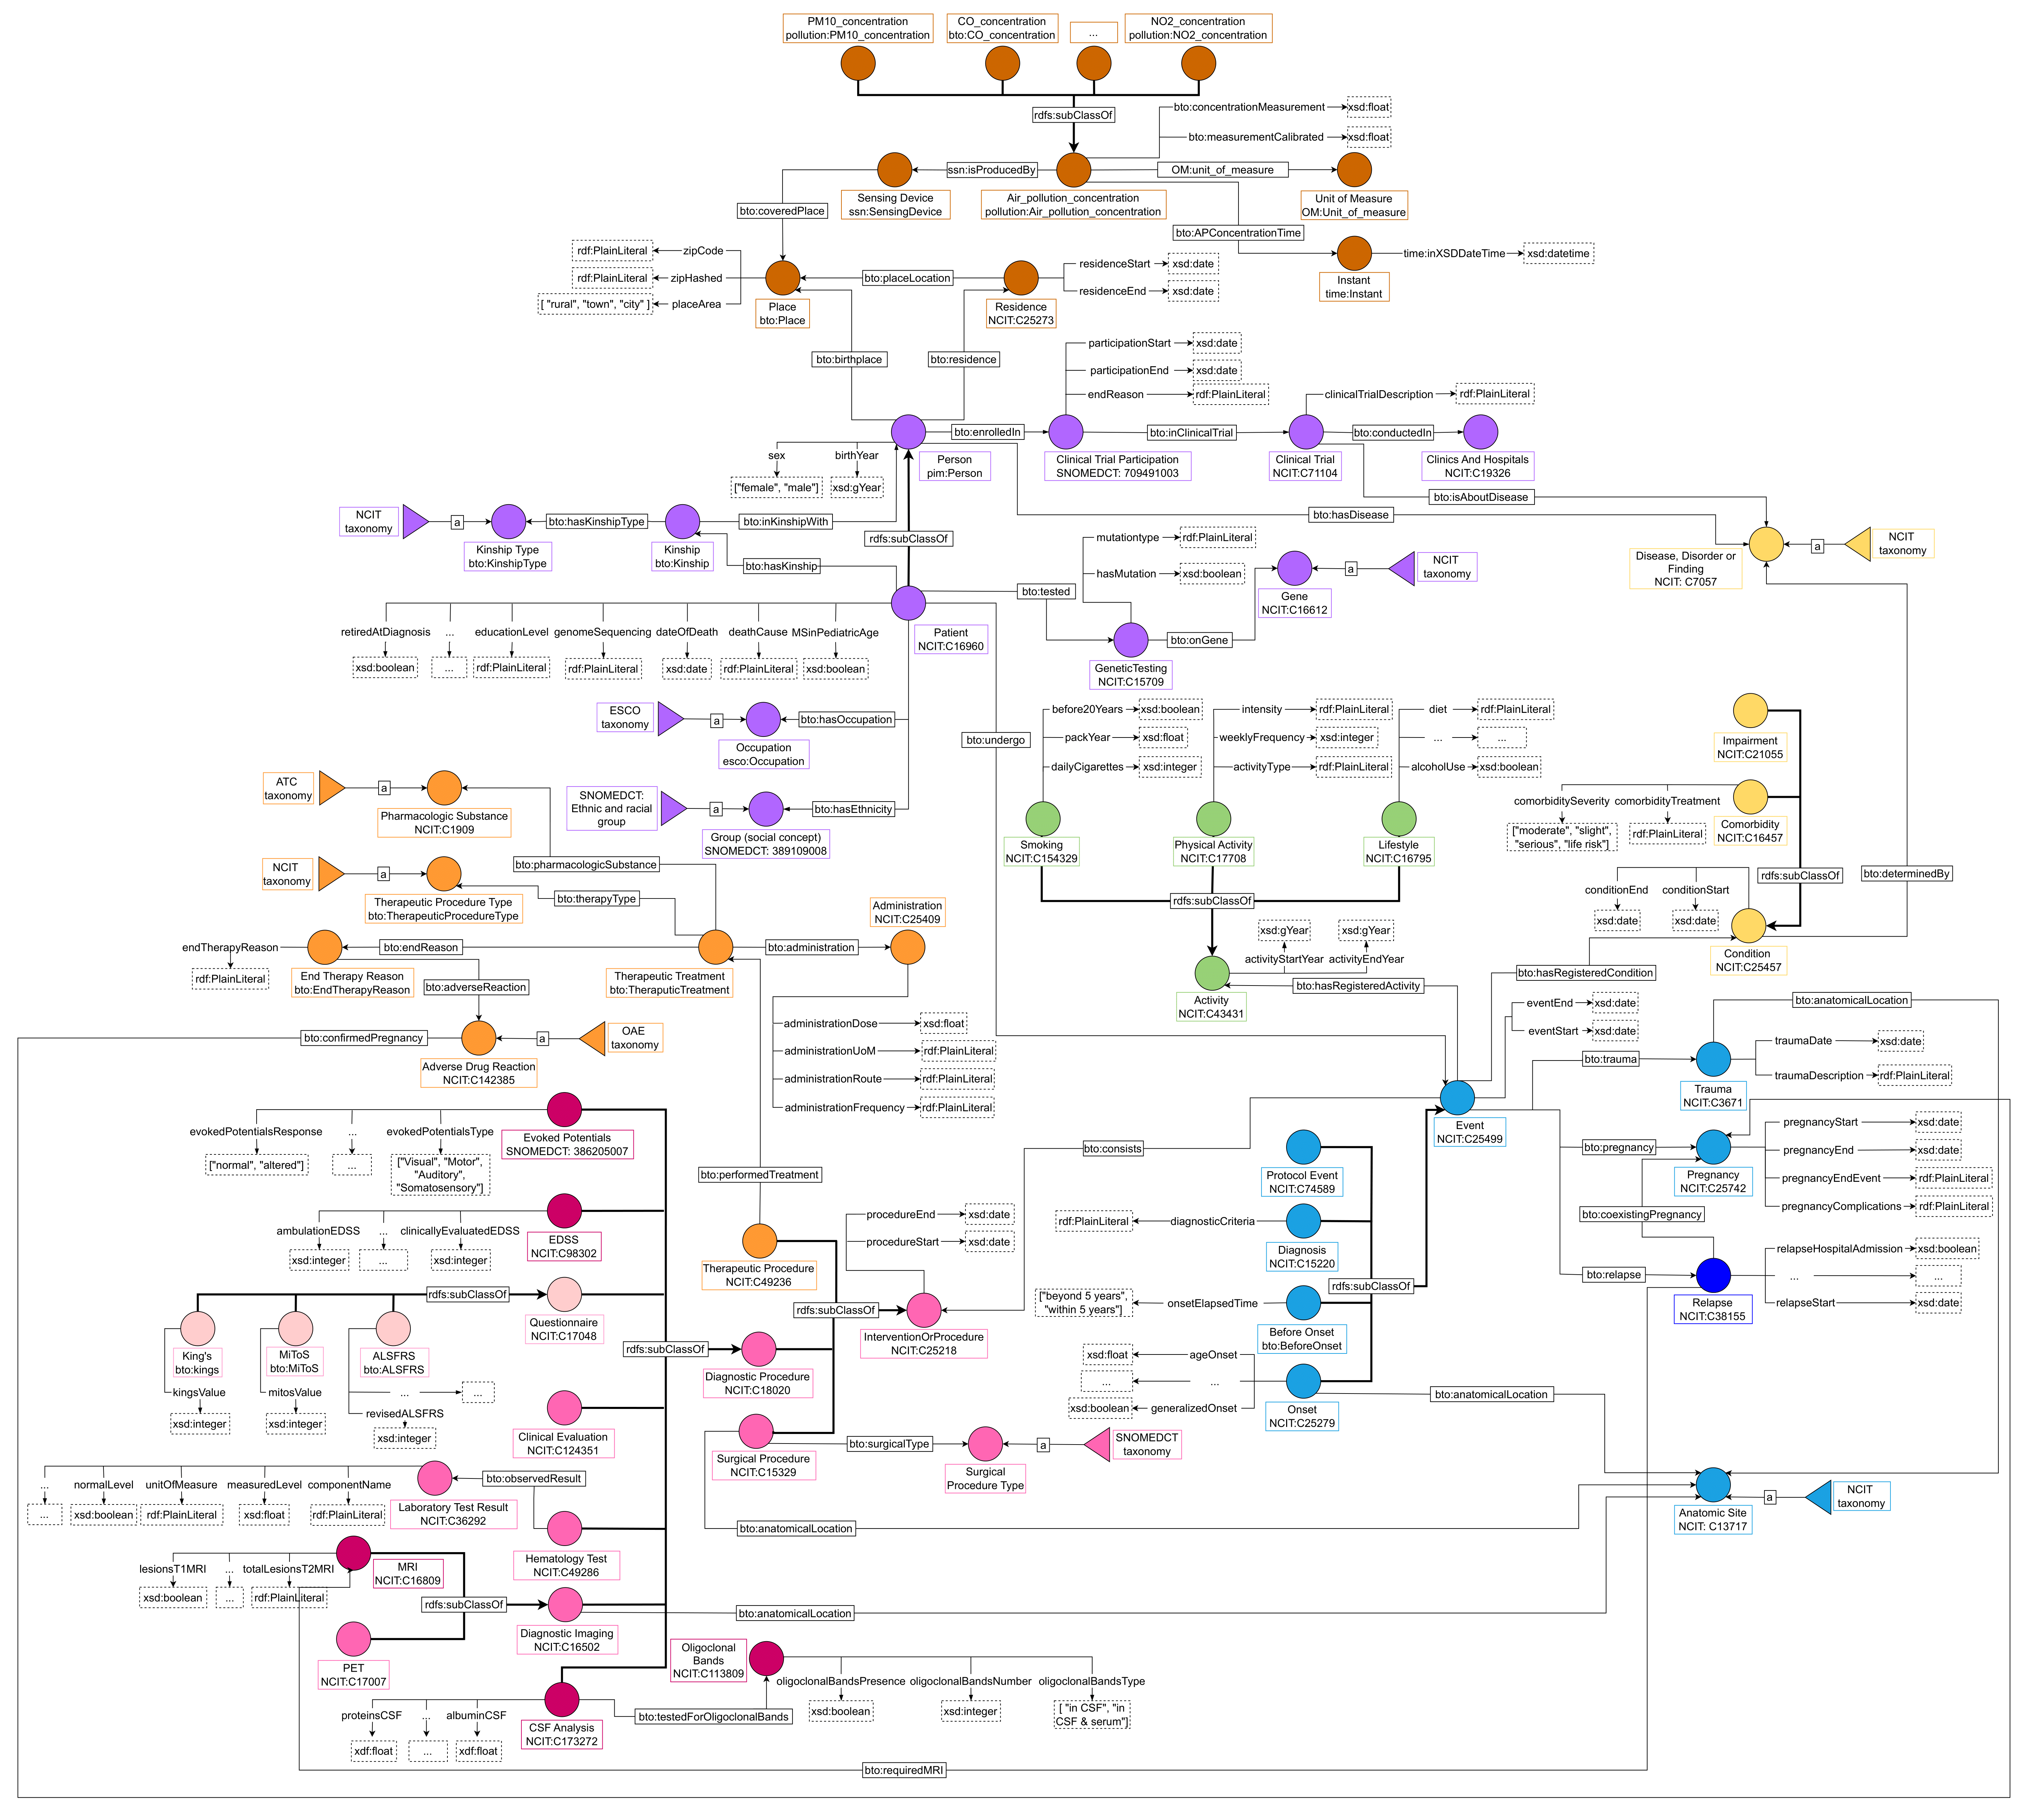
\includegraphics[width=15cm]{res/brainteaser.png}
  \caption{The Brainteaser Ontology}
  \label{fig:bto}
\end{figure}
\subsection{Ontology Features and Capabilities}
The Brainteaser Ontology models meticulously various aspects of patient health data, including genetic markers, clinical symptoms, diagnostic test results, and treatment responses. This comprehensive modeling approach ensures that all relevant data dimensions are captured and can be queried effectively. One of the key strengths of the Brainteaser Ontology is its focus on interoperability. It is built to integrate seamlessly with existing medical and genomic data standards, facilitating easy data exchange and compatibility with other health information systems. As new discoveries are made and healthcare practices evolve, the ontology is structured to be scalable and flexible. It can accommodate additional data types and relationships, supporting the ongoing growth and diversification of biomedical data.
\subsection{Ontology Implementation}
In our system, the Brainteaser Ontology acts as the vocabulary for designing semantic queries over data. By mapping our virtual data model with this ontology, we ensure that data from disparate sources can be integrated coherently and that complex queries involves all data coming from the heterogeneous data sources.

\section{OBDA Layer}
In our architecture, The component realizing the \ac{OBDA} paradigm, that aims to set up a \ac{VKG}, is Ontop.
Ontop comes in different shapes: different tools are provided for accomplishing different tasks.
In this section we will discuss the different Ontop tools that have been employed in our project alongside their actual role, with also code examples.
\subsection{Ontop Mapping}
Protégé is a well-known tool for ontology modelling, developed and maintained by the Stanford University. Apart from its standard capabilities, it is open to custom plugins that can be installed on demand, that expand its features.
To develop ontology mappings between an ontology and a single relational data source, as in the \ac{OBDA} paradigm is defined, the Ontop Mappings plugin for Protégé have been realized. Its utilization process is defined as follows:
\begin{itemize}
  \item The ontology that has to be mapped has to be opened with Protégé;
  \item The Ontop Mappings plugin has three tabs: the first one is about setting up the \ac{JDBC} connection with the relational source (i.e. Dremio). The \ac{JDBC} driver has to be manually loaded within the Protégé "connectors" folder;
  \item The second tab is about defining Ontop properties. For the mapping task, no specific property needs to be defined;
  \item The third tab is the mappings editor. Here, there are two different input fields: one asks for a portion of the graph, in Turtle notation, with autocomplete features; the second one is about the SQL query against the relational sources. Rows coming from the relational sources are directly mapped by including fields name within curly brackets in the Turtle syntax. Note that if there are mistakes in the Turtle notation (e.g. the subgraph doesn't match with the ontology), the mapping can't be added.
  \item After defining all mappings, they can be validated by clicking on "Validate". \ac{SQL} queries are executed and if they are wrong, or field names doesn't coincide with the one defined within curly brackets, an exception is raised;
  \item By saving the Protégé project, an .obda file is created in the ontology folder, containing mappings definition.
\end{itemize}  

For shortness, a portion of the mappings implementation between the virtual relational schema exposed by Dremio and the Brainteaser Ontology is shown in Code \ref{lst:mappings}.

\begin{lstlisting}[language=OntopNative, caption={Mappings definition between the virtual relational schema exposed by Dremio and the Brainteaser Ontology}, label={lst:mappings}]
  [MappingDeclaration] @collection [[
  mappingId	MAPID-5b34961b80264140bb779dbd296424ac
  target		bto:Patient{patient} a bto:Patient . 
  source		SELECT patient FROM "@mirco.cazzaro"."STATIC_VARS";

  mappingId	MAPID-f24debb89dc84f73a47acdf763ec0b4f
  target		bto:Patient{patient} bto:alive {alive}^^xsd:boolean . 
  source		SELECT patient, LCASE(alive) AS alive
        FROM "@mirco.cazzaro"."STATIC_VARS"
        WHERE alive <> '';

  mappingId	MAPID-5b2c0dfea75d44279ce8ddde95f2a9aa
  target		bto:Patient{patient} bto:sex {sex}^^xsd:string . 
  source		SELECT patient, LCASE(sex) AS sex
        FROM "@mirco.cazzaro"."STATIC_VARS"
        WHERE sex <> '';

  mappingId	MAPID-51a6eb8de7c64b7bbe4fe62d8188208c
  target		bto:Patient{patient} bto:undergo bto:eventOnset1{patient} . bto:eventOnset1{patient} a bto:Onset ; bto:eventStart {onsetDate}^^xsd:datetime ; bto:bulbarOnset {onset_bulbar}^^xsd:boolean ; bto:axialOnset {onset_axial}^^xsd:boolean ; bto:generalizedOnset {onset_generalized}^^xsd:boolean ; bto:limbsOnset {onset_limbs}^^xsd:boolean . 
  source		SELECT patient, onsetDate, LCASE(onset_bulbar) AS onset_bulbar, LCASE(onset_axial) AS onset_axial, LCASE(onset_generalized) AS onset_generalized, LCASE(onset_limbs) AS onset_limbs FROM "@mirco.cazzaro"."STATIC_VARS";

  mappingId	MAPID-541428e7a83441f5bd29e52d66ffc52e
  target		bto:Patient{patient} bto:undergo bto:eventOnset2{patient} . bto:eventOnset2{patient} a bto:Onset ; bto:ageOnset {age_onset}^^xsd:float . 
  source		SELECT patient, age_onset FROM "@mirco.cazzaro"."STATIC_VARS" WHERE age_onset <> '';

  mappingId	MAPID-ff2b4bdc90af468793b4f58105fa555f
  target		bto:Patient{patient} bto:undergo bto:diagnosis{patient} . bto:diagnosis{patient} a bto:Diagnosis ; bto:eventStart {diagnosisDate}^^xsd:datetime . 
  source		SELECT patient, diagnosisDate FROM "@mirco.cazzaro"."STATIC_VARS";

  mappingId	MAPID-13ab39d8b67c4f34a206b7f4bcc1f442
  target		bto:Patient{patient} bto:hasEthnicity bto:eth{patient} . bto:eth{patient} rdfs:label {ethnicity}@en . 
  source		SELECT patient, ethnicity FROM "@mirco.cazzaro"."STATIC_VARS" WHERE ethnicity <> '';

  mappingId	MAPID-56da0e23dc6b4cb3a0bfc475f4bcb65f
  target		bto:eventOnset3{patient} bto:anatomicalLocation bto:location{patient} . bto:location{patient} rdfs:label {onset_location}^^xsd:string . 
  source		SELECT patient, onset_location FROM "@mirco.cazzaro"."STATIC_VARS" WHERE onset_location <> '';

  mappingId	MAPID-5ea1e8edbbb1446fb50e887c4f0605dd
  target		bto:eventOnset4{patient} bto:consists bto:clinicalEvaluation{patient} . bto:clinicalEvaluation{patient} a bto:ClinicalEvaluation ; bto:predominantLimbsSide {onset_limbs_side}^^xsd:string ; bto:predominantLimbsImpairment {onset_limbs_impairment}^^xsd:string . 
  source		SELECT patient, onset_limbs_side, onset_limbs_impairment
        FROM "@mirco.cazzaro"."STATIC_VARS"
        WHERE onset_limbs_side <> '' OR onset_limbs_impairment <> '';
  ]]
\end{lstlisting}

\subsection{Ontop SPARQL}
The aim of the OBDA approach is executing \ac{SPARQL} queries over a \ac{VKG}. Testing mapping correctness before their utilization in a running environment is essential. The Ontop SPARQL plugin for Protégé accomplishes this task. Given its role of a testing tool, it allows to analyze the "\ac{SQL} translation" of the running \ac{SPARQL} query.
\subsection{Ontop Endpoint}
The Ontop Standalone Endpoint provides a server environment where Ontop can operate independently, offering both an API and a web interface for running SPARQL queries over the virtual knowledge graph. This setup is particularly useful for environments where integration with existing data management systems is necessary, .
\subsection{Ontop with GraphDB}

    %!TEX root = ../main.tex

\chapter{Use Cases}
\label{chp:usecase}
    %!TEX root = ../main.tex

\chapter{Evaluation Results}
\label{chp:evaluation}
    %!TEX root = ../main.tex

\chapter{Conclusions and Future Works}
\label{chp:conclusions}


    
    % Bibliography, appendix, acknowledges, etc...
    \backmatter
\end{document}